\documentclass[journal]{IEEEtran}

\usepackage{amsmath,amssymb,amsfonts}
\usepackage{graphicx}
\usepackage{booktabs}
\usepackage{cite}
\usepackage{url}
\usepackage{array}
\usepackage{multirow}
\usepackage{balance}
\usepackage{tikz}
\usetikzlibrary{arrows.meta,positioning,shapes.geometric,fit}

\graphicspath{{figures/source_from_dissertation/}{figures/generated/}}

\newcommand{\E}{\mathcal{E}}
\newcommand{\D}{\mathcal{D}}
\newcommand{\T}{\mathcal{T}}
\newcommand{\C}{\mathcal{C}}
\newcommand{\BA}{\mathrm{BA}}
\newcommand{\AUC}{\mathrm{AUC}}
\newcommand{\R}{\mathbb{R}}

\begin{document}

\title{Operational Distinctness in Staged Neuromorphic Architectures: A Layer Ablation Analysis of Clinical EEG}

\author{Andrew A. Lane, K. Wendy Tang, and Brady D. Nelson%
\thanks{This manuscript draft was generated from corrected, privacy-preserving reporting outputs at commit \texttt{bcafc50ca544da35ee215f030849a34bfb395a4c}. Clinical-label findings are interpreted as exploratory sensitivity analyses because permutation-FDR inference was not completed in the current run.}%
}

\maketitle

\begin{abstract}
Hybrid biomedical signal-processing architectures increasingly combine temporal encoders, graph modules, dynamical descriptors, and interpretability layers. In electroencephalography (EEG), however, endpoint classification accuracy alone cannot determine whether these stages perform distinct operations or merely re-express redundant information. This paper evaluates \emph{operational distinctness} in Affective Reservoir-Spike Processing and Inference Network (ARSPI-Net), a staged neuromorphic architecture for clinical affective EEG. ARSPI-Net maps multichannel event-related EEG into four derived feature families: a binned spike-count reservoir embedding $E$, reservoir-response dynamical descriptors $D$, graph-topological descriptors $T$, and structure-function coupling features $C$. Using 633 subject-condition observations from 211 subjects and 34 channels, we evaluate a controlled ablation matrix under subject-safe cross-validation. For three-class affective condition classification, $E$ alone achieved 46.96\% balanced accuracy and 0.6460 macro one-versus-rest ROC-AUC; embedding-containing combinations were strongest, with $E+D$ reaching 49.34\% balanced accuracy and $E+D+T$ reaching 0.6549 macro ROC-AUC, comparable to the band-power baseline at 49.27\% balanced accuracy and 0.6783 macro ROC-AUC. Exploratory clinical-label sensitivity showed a different layer profile: SUD peaked in $E+D+T$ (56.46\%, AUC 0.6019), MDD in $E$ (52.35\%, AUC 0.5586), PTSD in $D+T$ (52.87\%, AUC 0.5294), GAD in $T$ (51.64\%, AUC 0.5295), and ADHD in $D+T$ (55.21\%, AUC 0.5559). Pairwise centered-kernel alignment values were low to moderate, with the largest CKA between $E$ and $D$ (0.3058). These results support a target-dependent measurement interpretation: ARSPI-Net layers are not a simple accuracy-increasing stack; they expose non-equivalent temporal, dynamical, topological, and cross-scale views of the same EEG response. Clinical results remain exploratory and do not establish diagnostic biomarkers.
\end{abstract}

\begin{IEEEkeywords}
EEG, neuromorphic computing, spiking neural networks, liquid state machines, reservoir computing, graph neural networks, clinical-label sensitivity, layer ablation, operational distinctness.
\end{IEEEkeywords}

\section{Introduction}
Electroencephalography (EEG) provides millisecond-scale access to neural activity, but scalp recordings are noisy, indirect, subject-dependent observations of latent neural dynamics. Clinical affective EEG is particularly difficult because affective stimulus responses, inter-subject covariance, comorbidity, medication, and nonstationarity coexist in the same measurement. A single endpoint classifier can be useful, but it does not by itself determine which component of a staged architecture carries information, whether later layers add discriminative utility, or whether intermediate representations measure distinct signal properties.

Recent IEEE biomedical and neural-systems papers set a high methodological bar for EEG architectures. Compact EEG convolutional baselines such as EEGNet~\cite{lawhern2018eegnet}, EEG graph neural networks~\cite{klepl2024gnn,klepl2023ad}, and spiking/graph hybrids~\cite{gong2023sglnet} are typically evaluated through cross-subject protocols, ablations, multiple metrics, and architectural diagrams. Biomedical informatics studies similarly report modality-specific comparisons, ablation logic, and cross-subject validation when proposing physiological classifiers~\cite{guo2025mma,chiang2023depression}. These papers highlight a standard that the present study follows: a staged architecture is not adequately justified by a single final accuracy value. Its modules must be evaluated by what they contribute.

This paper studies this problem in Affective Reservoir-Spike Processing and Inference Network (ARSPI-Net), a staged neuromorphic EEG architecture. ARSPI-Net maps each event-related EEG observation into several feature families: a reservoir spike embedding $E$, dynamical descriptors $D$, graph-topological descriptors $T$, and structure-function coupling descriptors $C$. Earlier ARSPI-Net manuscripts addressed different questions: one characterized subject-covariance structure, and another defined a four-level interpretability framework. The present manuscript asks a more architectural question: are the ARSPI-Net layers operationally distinct, or are they redundant feature blocks?

We define operational distinctness as empirical non-equivalence of layers under a fixed evaluation protocol. A layer may be operationally distinct if it differs in predictive sufficiency, incremental utility, clinical-label sensitivity, or representational redundancy. This definition is intentionally measurement-oriented. It does not assert that layers correspond to independent biological mechanisms. It asks whether they behave as different signal-processing views of the same EEG response.

The contributions are fourfold:
\begin{enumerate}
    \item We formalize a layer-ablation test for staged neuromorphic EEG architectures.
    \item We evaluate ARSPI-Net feature families $E$, $D$, $T$, and $C$ under a controlled A0--A9 affective ablation and C1--C6 clinical-label sensitivity matrix.
    \item We report feature diagnostics, redundancy analysis, and comorbidity-adjusted exploratory models to constrain claim strength.
    \item We distinguish predictive utility from measurement utility, showing that ARSPI-Net layers are target-dependent rather than a monotonic accuracy stack.
\end{enumerate}

\section{Related Work and Novelty Boundary}
\subsection{EEG Classification and Biomedical Evaluation Norms}
EEG classification papers commonly compare new representations against compact neural baselines, spectral features, recurrent models, and graph-based models~\cite{lawhern2018eegnet,craik2019deep,klepl2024gnn}. In TNSRE, Gong \emph{et al.} integrated spike encoding, adaptive graph convolution, and spike-based LSTM units for EEG-based BCI and reported cross-subject evaluation, parameter analysis, and confusion matrices~\cite{gong2023sglnet}. In JBHI, Guo \emph{et al.} proposed a multimodal attention network for EEG/EDA/PPG fatigue detection and reported cross-subject experiments and modality comparisons~\cite{guo2025mma}. These examples motivate the present manuscript's structure: architecture, mathematical definition, controlled ablation, multiple metrics, claim-bounded clinical discussion, and reproducible outputs.

\subsection{Graph and Spiking EEG Models}
Graph neural networks have been used for emotion recognition, motor imagery, and neurological or psychiatric classification from EEG. Klepl \emph{et al.} emphasized that EEG-GNN methods differ substantially in node features, graph construction, graph convolution, pooling, and readout choices~\cite{klepl2024gnn}. Spiking methods add temporal event-based computation and dynamical state variables~\cite{maass2002liquid,gong2023sglnet}. ARSPI-Net differs from end-to-end EEG classifiers by treating the reservoir as a fixed nonlinear measurement operator whose outputs support multiple downstream descriptors.

\subsection{Novelty Boundary Relative to Prior ARSPI-Net Work}
The novelty of this paper is not the mere existence of ARSPI-Net, nor the claim that ARSPI-Net is interpretable. The unique question is whether the feature families generated by ARSPI-Net behave as distinct operational layers. Fig.~\ref{fig:novelty_boundary} summarizes this boundary.

\begin{figure}[!t]
\centering
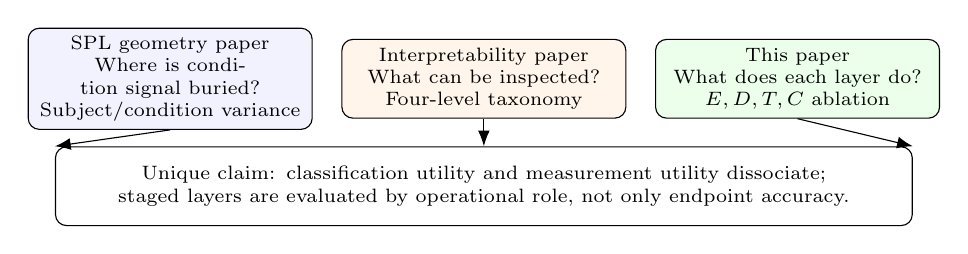
\begin{tikzpicture}[font=\scriptsize, node distance=0.12cm]
\tikzstyle{blk}=[draw, rounded corners, align=center, minimum height=1.0cm, inner sep=3pt]
\node[blk, fill=blue!5, text width=0.28\columnwidth] (spl) {SPL geometry paper\\ Where is condition signal buried?\\ Subject/condition variance};
\node[blk, fill=orange!8, text width=0.28\columnwidth, right=0.03\columnwidth of spl] (interp) {Interpretability paper\\ What can be inspected?\\ Four-level taxonomy};
\node[blk, fill=green!8, text width=0.28\columnwidth, right=0.03\columnwidth of interp] (this) {This paper\\ What does each layer do?\\ $E,D,T,C$ ablation};
\node[blk, fill=white, text width=0.88\columnwidth, below=0.35cm of interp] (claim) {Unique claim: classification utility and measurement utility dissociate; staged layers are evaluated by operational role, not only endpoint accuracy.};
\draw[-{Latex[length=2mm]}] (spl.south) -- (claim.north west);
\draw[-{Latex[length=2mm]}] (interp.south) -- (claim.north);
\draw[-{Latex[length=2mm]}] (this.south) -- (claim.north east);
\end{tikzpicture}
\caption{Novelty boundary relative to prior ARSPI-Net manuscripts. The present paper is a layer-role audit, not a repetition of subject-covariance geometry or a four-level interpretability taxonomy.}
\label{fig:novelty_boundary}
\end{figure}

\section{ARSPI-Net Layer Formulation}
\subsection{Input Representation}
Let
\begin{equation}
X_s^{(c)} \in \mathbb{R}^{N_{ch}\times T}, \qquad N_{ch}=34,
\end{equation}
denote the preprocessed event-related EEG response for subject $s$ under condition $c\in\{\mathrm{negative},\mathrm{neutral},\mathrm{pleasant}\}$. The affective task uses subject-condition observations; clinical-label analyses average each feature family over the available conditions for each subject.

\subsection{Reservoir Dynamics and Spike Embedding}
For each channel, a fixed leaky-integrate-and-fire (LIF) reservoir transforms the input waveform into membrane trajectories and spike trains. A discrete-time LIF reservoir update is
\begin{equation}
\mathbf{u}_{t+1}=\beta\mathbf{u}_{t}+W_{in}x_t+W_{rec}\mathbf{z}_t-\mathbf{r}_t,
\label{eq:lif}
\end{equation}
with spike emission
\begin{equation}
\mathbf{z}_{t+1}=H(\mathbf{u}_{t+1}-\theta),
\label{eq:spike}
\end{equation}
where $H(\cdot)$ is the Heaviside step function, $\beta=0.05$ is the membrane decay, $\theta=0.5$ is the threshold, and $W_{in}$ and $W_{rec}$ are fixed matrices. Binned spike counts over six temporal windows produce BSC$_6$ features. After PCA compression to 64 components per channel, the embedding is
\begin{equation}
E_s^{(c)}=\left[h_1^{(0)}\|h_2^{(0)}\|\cdots\|h_{34}^{(0)}\right]\in\mathbb{R}^{2176},
\label{eq:E}
\end{equation}
where $h_v^{(0)}\in\mathbb{R}^{64}$ denotes the channel-level embedding.

\subsection{Dynamical, Topological, and Coupling Blocks}
The dynamical block $D$ contains reservoir-response descriptors over channels. The graph-topological block $T$ summarizes electrode-level topology. The coupling block $C$ summarizes the relation between dynamics and topology. For channel-wise matrices $D_s\in\mathbb{R}^{34\times p}$ and $T_s\in\mathbb{R}^{34\times q}$, a rank-correlation coupling matrix is
\begin{equation}
K_s = \mathrm{corr}_{\rho}(D_s,T_s) \in \mathbb{R}^{p\times q}.
\end{equation}
The normalized coupling magnitude is
\begin{equation}
\kappa_s = \frac{\|K_s\|_F}{\sqrt{pq}},
\label{eq:kappa}
\end{equation}
and the final $C$ block contains $\kappa_s$ and signed summaries of strength and clustering coupling.

\subsection{Operational Distinctness Criteria}
For feature families $L_i,L_j\in\{E,D,T,C\}$ and target $Y$, define the performance contrast
\begin{equation}
\Delta_{ij}(Y)=\mathcal{M}(f(L_i),Y)-\mathcal{M}(f(L_j),Y),
\label{eq:contrast}
\end{equation}
where $\mathcal{M}$ is balanced accuracy or ROC-AUC and $f$ is the fixed readout. Incremental utility relative to a baseline $L_b$ is
\begin{equation}
\Gamma_i(Y|L_b)=\mathcal{M}(f([L_b\|L_i]),Y)-\mathcal{M}(f(L_b),Y).
\label{eq:increment}
\end{equation}
Redundancy is assessed using linear centered-kernel alignment (CKA),
\begin{equation}
\mathrm{CKA}(X,Y)=\frac{\|X_c^{\top}Y_c\|_F^2}{\|X_c^{\top}X_c\|_F\|Y_c^{\top}Y_c\|_F},
\label{eq:cka}
\end{equation}
where $X_c$ and $Y_c$ are column-centered feature matrices~\cite{kornblith2019similarity}.

\section{Experimental Protocol}
\subsection{Data, Splitting, and Privacy}
The final reporting run used 633 observations from 211 subjects, exactly balanced across the three affective conditions. Clinical-label analyses used 206 subjects with available clinical labels. All prediction-level artifacts used hashed subject identifiers only. Raw EEG, clinical metadata, and feature pickles were not committed to the reporting repository.

Fig.~\ref{fig:protocol} summarizes the evaluation protocol. This figure is generated for the present manuscript and is separate from dissertation-source architecture figures.

\begin{figure*}[!t]
\centering
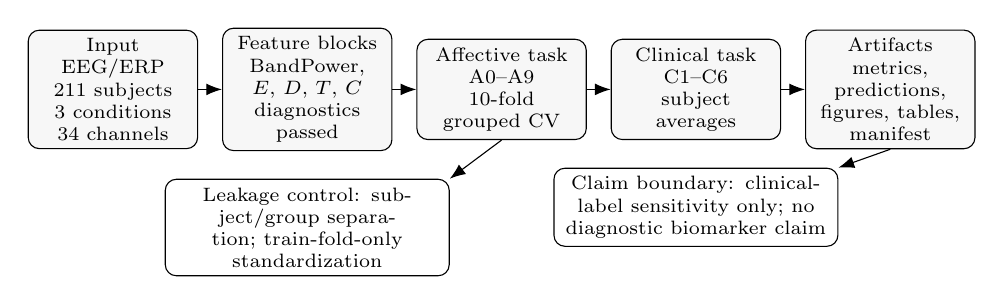
\begin{tikzpicture}[font=\scriptsize, node distance=0.16cm]
\tikzstyle{stage}=[draw, rounded corners, align=center, minimum height=0.9cm, inner sep=3pt, fill=gray!6]
\node[stage, text width=0.16\textwidth] (s1) {Input EEG/ERP\\211 subjects\\3 conditions\\34 channels};
\node[stage, text width=0.16\textwidth, right=0.025\textwidth of s1] (s2) {Feature blocks\\BandPower, $E$, $D$, $T$, $C$\\diagnostics passed};
\node[stage, text width=0.16\textwidth, right=0.025\textwidth of s2] (s3) {Affective task\\A0--A9\\10-fold grouped CV};
\node[stage, text width=0.16\textwidth, right=0.025\textwidth of s3] (s4) {Clinical task\\C1--C6\\subject averages};
\node[stage, text width=0.16\textwidth, right=0.025\textwidth of s4] (s5) {Artifacts\\metrics, predictions, figures, tables, manifest};
\foreach \x/\y in {s1/s2,s2/s3,s3/s4,s4/s5}{\draw[-{Latex[length=2mm]}] (\x) -- (\y);}
\node[stage, fill=white, text width=0.28\textwidth, below=0.35cm of s2] (l1) {Leakage control: subject/group separation; train-fold-only standardization};
\node[stage, fill=white, text width=0.28\textwidth, below=0.35cm of s4] (l2) {Claim boundary: clinical-label sensitivity only; no diagnostic biomarker claim};
\draw[-{Latex[length=2mm]}] (s3.south) -- (l1.north east);
\draw[-{Latex[length=2mm]}] (s5.south) -- (l2.north east);
\end{tikzpicture}
\caption{Subject-level reporting protocol used for the operational-distinctness analysis. Feature extraction outputs were diagnosed, ablated under subject-safe cross-validation, and exported as metrics, predictions, figures, tables, and manifests.}
\label{fig:protocol}
\end{figure*}

\subsection{Source Figures and New Figures}
Two dissertation-source figures are retained to define the ARSPI-Net architecture and BSC$_6$ embedding lineage. New figures in this manuscript are generated from the corrected reporting outputs and visualize the operational-distinctness analysis.

\begin{figure*}[!t]
\centering
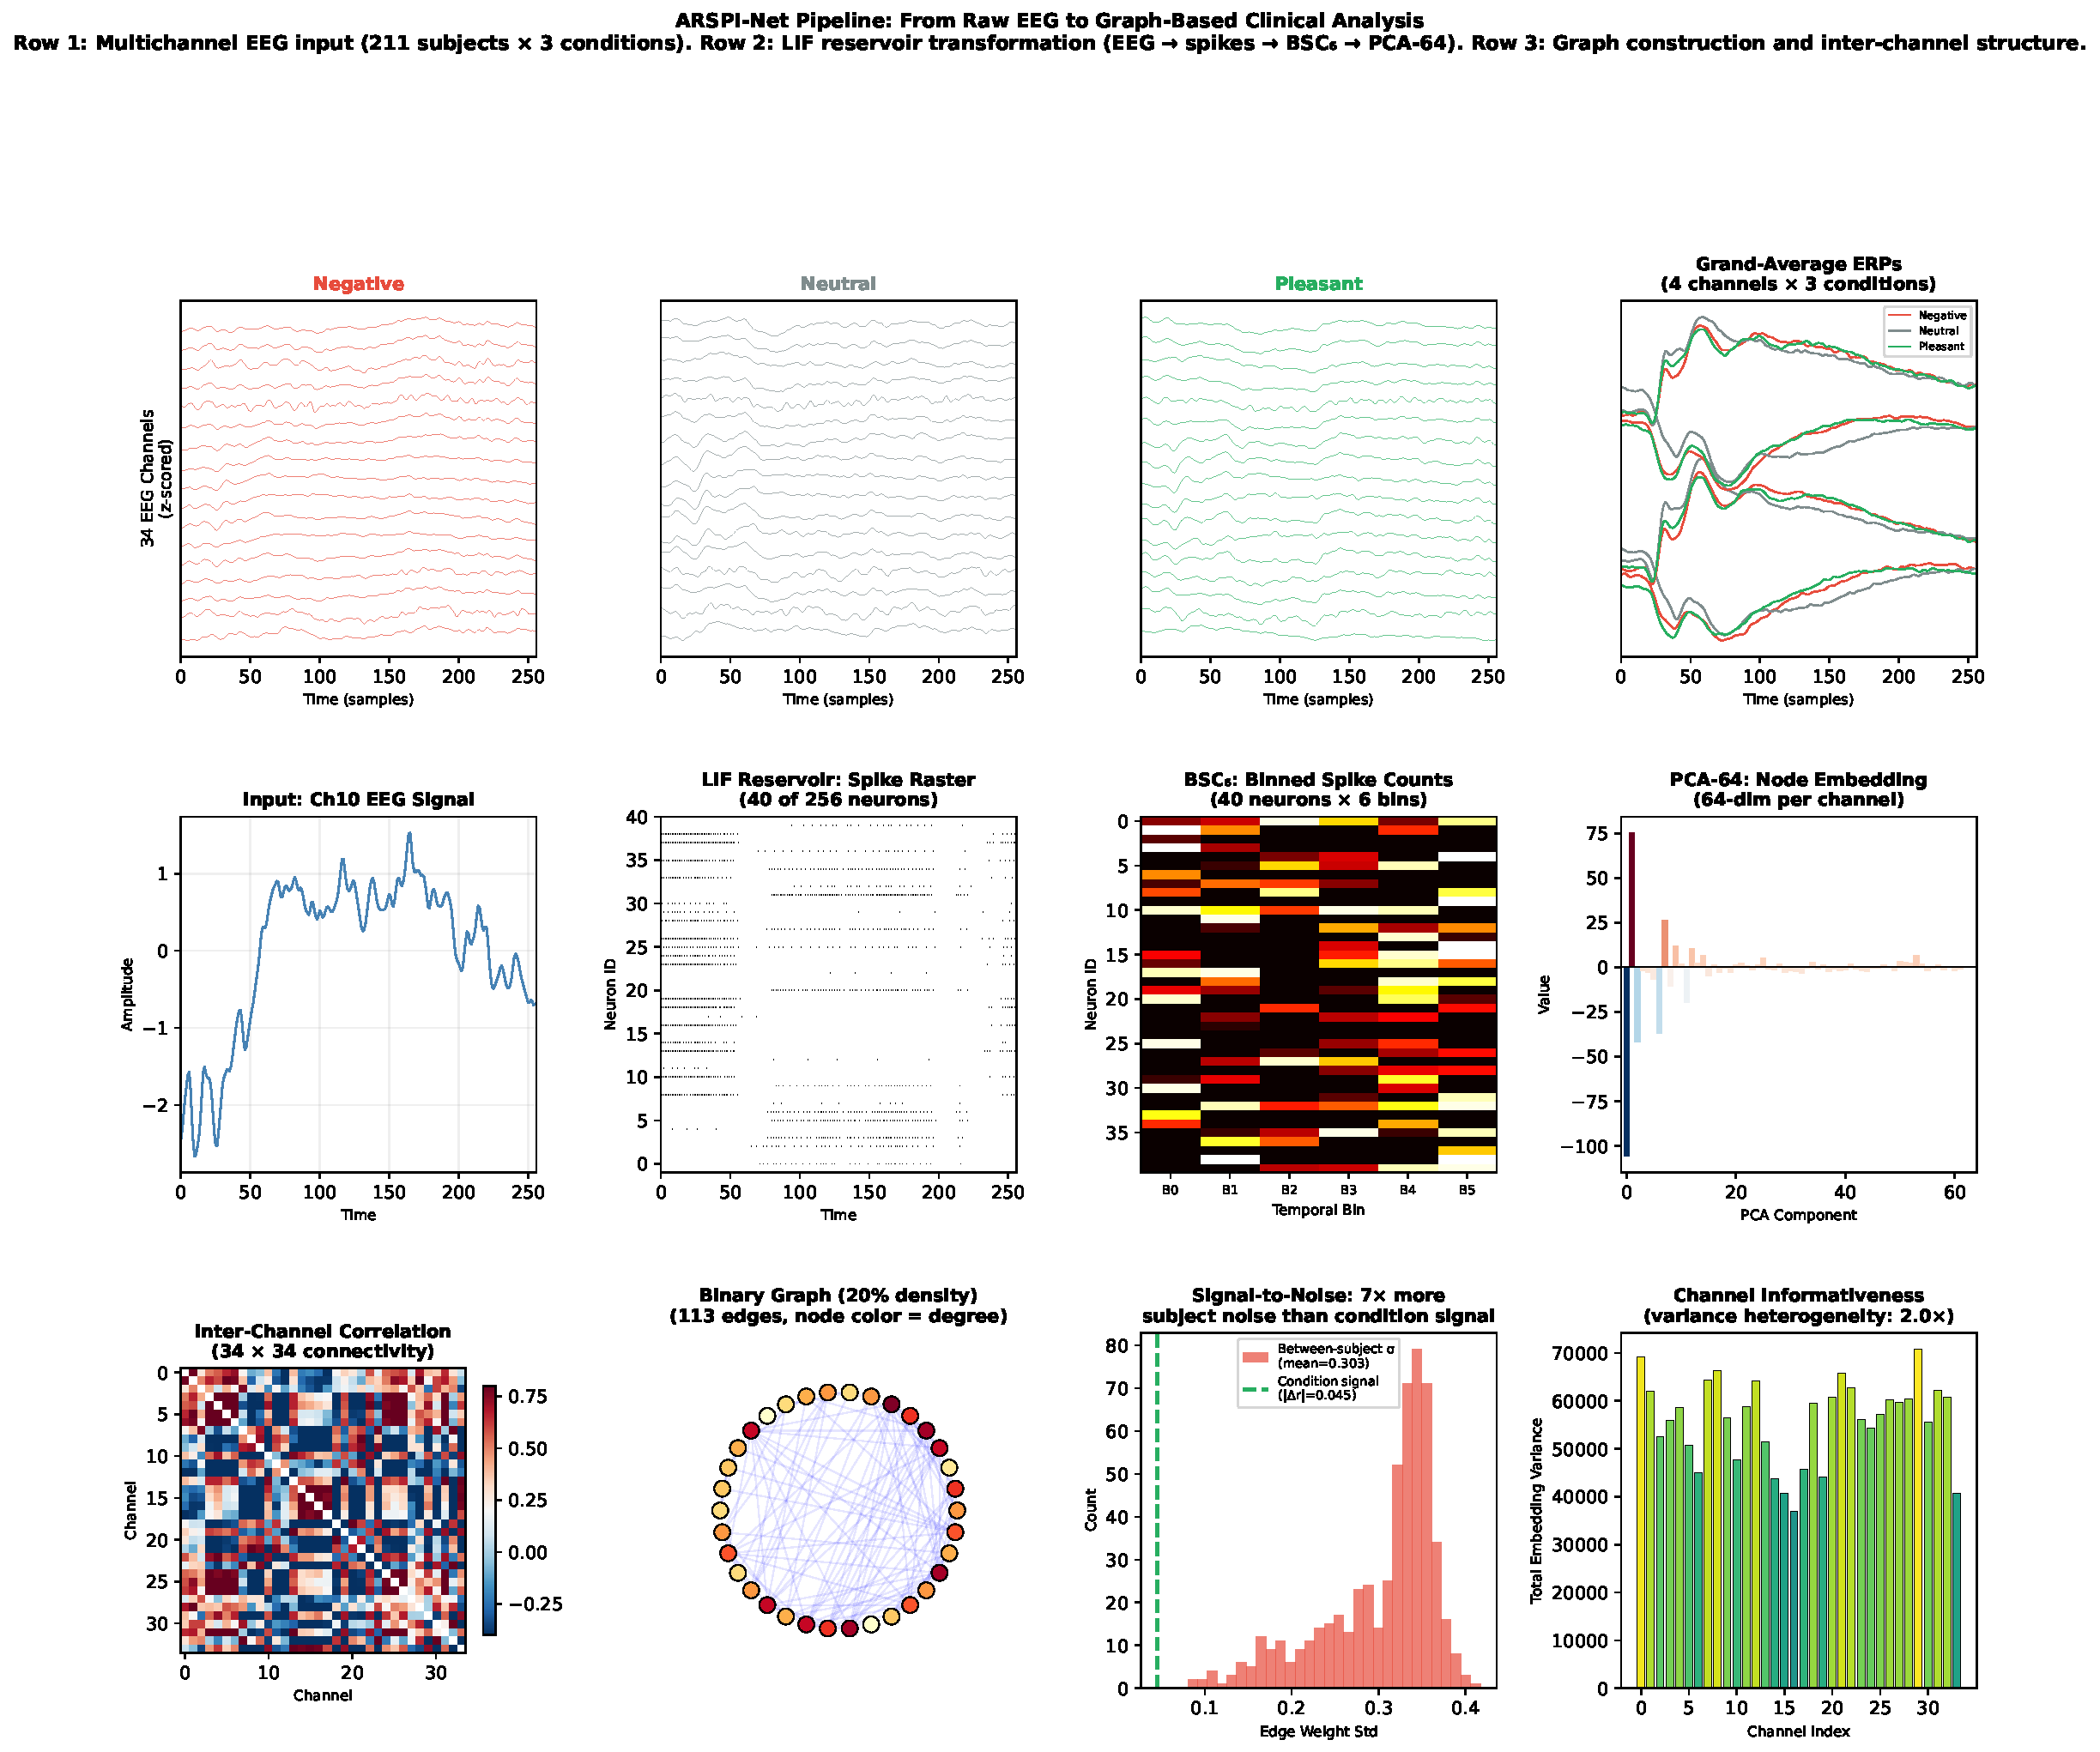
\includegraphics[width=0.98\textwidth]{dissertation_fig_pipeline_overview.pdf}
\caption{Dissertation-source ARSPI-Net pipeline overview. The figure defines the staged architecture whose layers are ablated in the present manuscript.}
\label{fig:source_pipeline}
\end{figure*}

\begin{figure*}[!t]
\centering
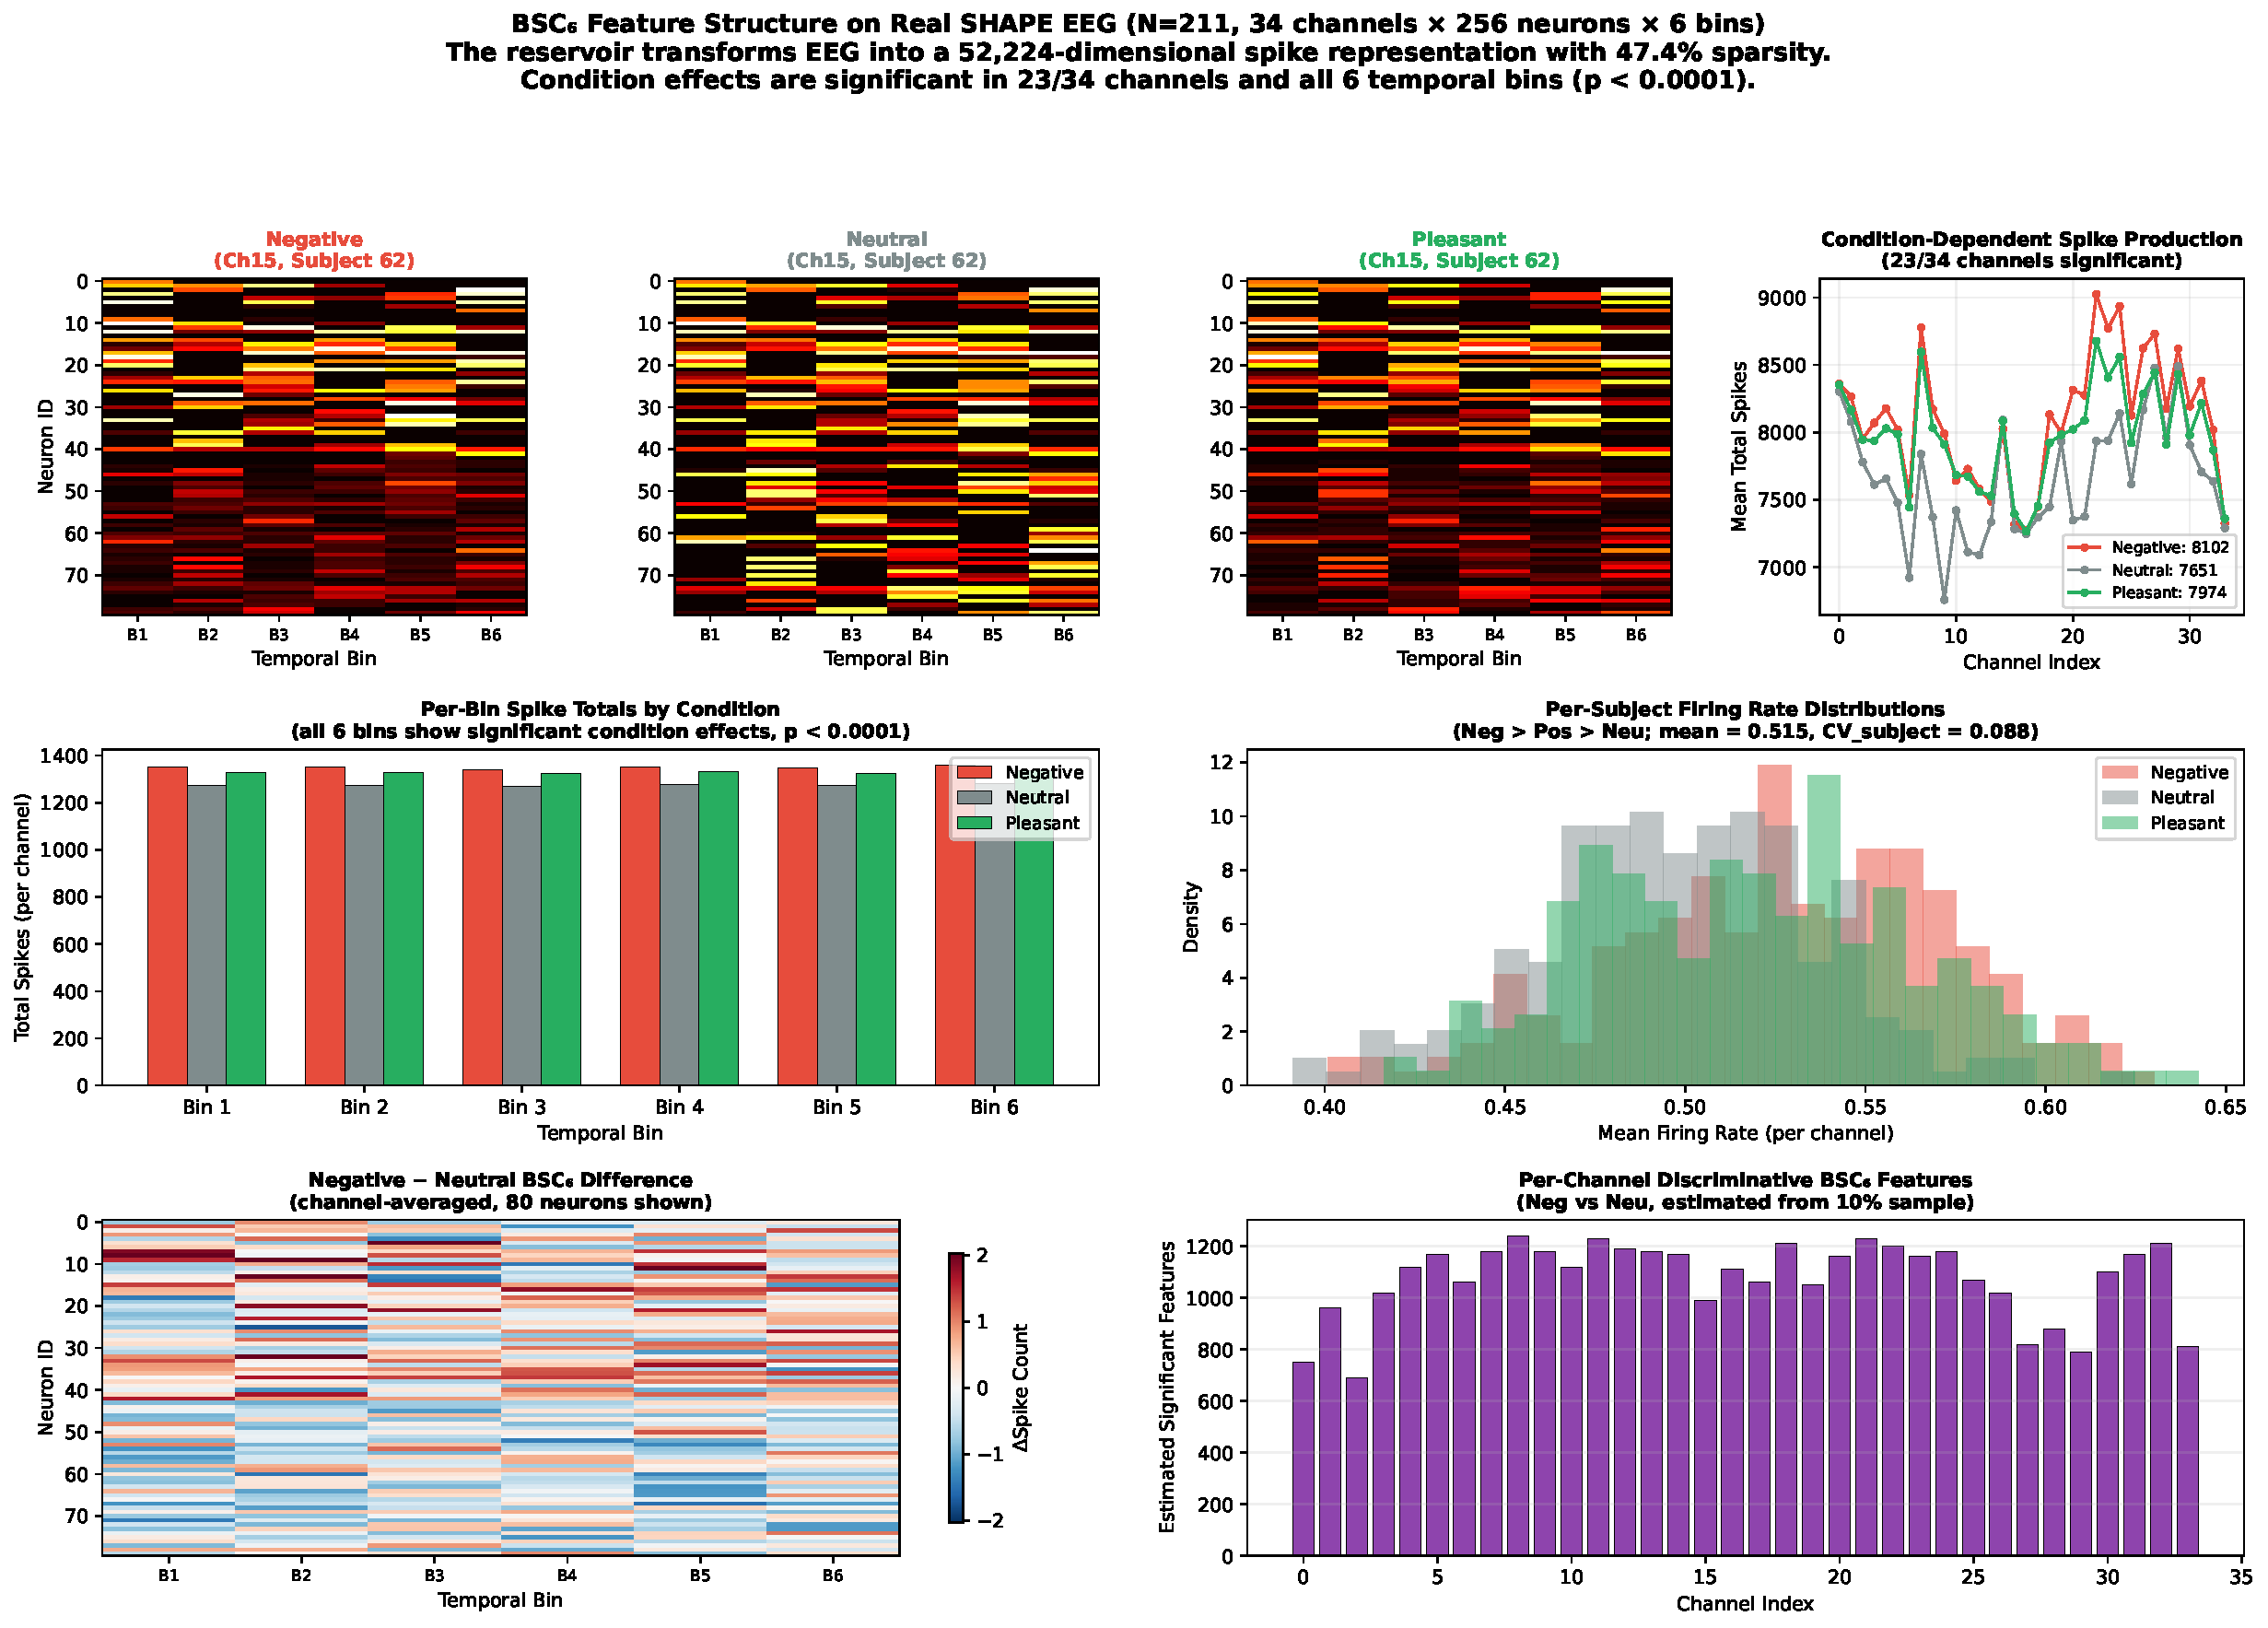
\includegraphics[width=0.98\textwidth]{dissertation_fig_bsc6_real_eeg.pdf}
\caption{Dissertation-source BSC$_6$ feature-structure figure for real SHAPE EEG. The quantitative results in this paper are generated from the corrected reporting pipeline, not manually transcribed from this source figure.}
\label{fig:bsc6_source}
\end{figure*}

\subsection{Feature Blocks and Diagnostics}
The evaluated feature blocks are listed in Table~\ref{tab:feature_blocks}. A feature diagnostic was run before interpretation. The corrected embedding $E$ had shape $(633,2176)$, no constant columns, zero fraction 0, approximate standardized rank 632, and median row norm 224.61. This diagnostic is reported because an earlier local input file contained a zero-valued embedding tensor; it was replaced before the final run.

\begin{table*}[!t]
\caption{Feature Families Used in the Operational-Distinctness Analysis}
\label{tab:feature_blocks}
\centering
\footnotesize
\begin{tabular}{llll}
\hline
Block & Dimension & Source & Operational role \\
\hline
BandPower & 170 & Spectral features & Conventional frequency-domain comparator \\
$E$ & 2176 & BSC$_6$/PCA-64 reservoir embedding & Temporal spike representation \\
$D$ & 238 & Reservoir trajectory descriptors & Dynamical response characterization \\
$T$ & 68 & Graph-topological descriptors & Spatial organization across electrodes \\
$C$ & 3 & Structure-function coupling & Alignment of dynamics and topology \\
\hline
\end{tabular}
\end{table*}


\subsection{Ablation Matrices}
Affective classification used A0--A9 configurations. The classifier was L2-regularized logistic regression with train-fold-only standardization and 10-fold StratifiedGroupKFold subject separation. Clinical-label sensitivity used C1--C6 configurations at the subject level. The readout was again logistic regression, enabling a stable linear separability analysis rather than an unconstrained nonlinear endpoint model.

The logistic objective is
\begin{equation}
\hat{\theta}=\arg\min_{\theta}\left[-\sum_{i=1}^{n}\log p_{\theta}(y_i|x_i)+\lambda\|\theta\|_2^2\right].
\label{eq:logreg}
\end{equation}
The primary metric is balanced accuracy,
\begin{equation}
\BA=\frac{1}{K}\sum_{k=1}^{K}\frac{TP_k}{TP_k+FN_k}.
\label{eq:ba}
\end{equation}
For clinical-label sensitivity, $K=2$; for affective classification, $K=3$.

\section{Results}
\subsection{Affective Ablation: Embedding-Containing Combinations Are Strongest}
Table~\ref{tab:affective_ablation} and Fig.~\ref{fig:affective_dual} report the corrected A0--A9 affective ablation. $E$ alone achieved 46.96\% balanced accuracy and 0.6460 macro ROC-AUC. $E+D$ had the highest balanced accuracy at 49.34\%, and $E+D+T$ had the highest macro ROC-AUC among ARSPI-Net configurations at 0.6549. The band-power baseline remained competitive, achieving 49.27\% balanced accuracy and 0.6783 macro ROC-AUC.

\begin{table}[!t]
\caption{Affective Condition Classification Across A0--A9 Configurations}
\label{tab:affective_ablation}
\centering
\footnotesize
\begin{tabular}{llcc}
\hline
Config. & Feature set & Balanced acc. & Macro ROC-AUC \\
\hline
A0 & BandPower & 0.4927 & 0.6783 \\
A1 & $E$ & 0.4696 & 0.6460 \\
A2 & $D$ & 0.4224 & 0.5977 \\
A3 & $T$ & 0.3534 & 0.5270 \\
A4 & $C$ & 0.3552 & 0.5417 \\
A5 & $D+T$ & 0.4381 & 0.6148 \\
A6 & $E+D$ & \textbf{0.4934} & 0.6520 \\
A7 & $E+T$ & 0.4725 & 0.6486 \\
A8 & $E+D+T$ & 0.4933 & \textbf{0.6549} \\
A9 & $E+D+T+C$ & 0.4933 & 0.6542 \\
\hline
\end{tabular}
\end{table}


\begin{figure*}[!t]
\centering
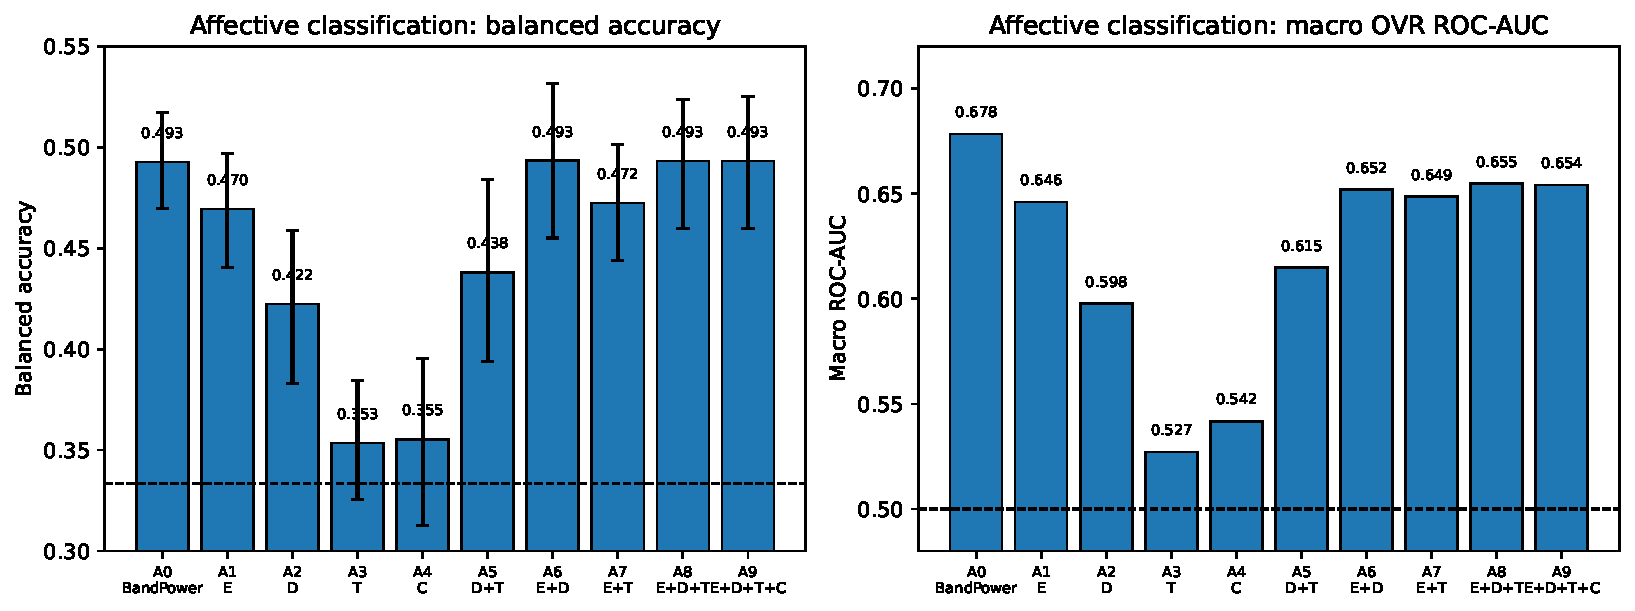
\includegraphics[width=0.98\textwidth]{fig04_affective_ablation_dual_metric.pdf}
\caption{Affective ablation results. Embedding-containing configurations provide the strongest balanced accuracies among ARSPI-Net representations, but remain comparable to the band-power baseline.}
\label{fig:affective_dual}
\end{figure*}

\begin{figure}[!t]
\centering
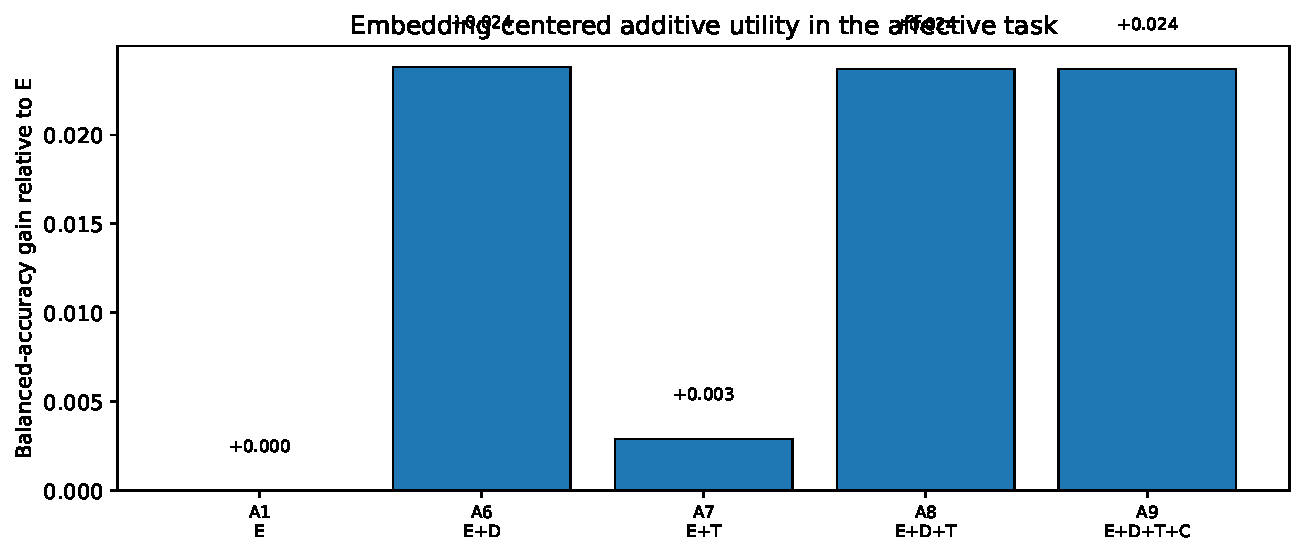
\includegraphics[width=\columnwidth]{fig05_embedding_additive_utility.pdf}
\caption{Embedding-centered additive utility for the affective task. Adding $D$ to $E$ gives the largest observed gain. Adding $C$ to $E+D+T$ does not improve balanced accuracy.}
\label{fig:additive}
\end{figure}

This result does not support a simplistic claim that every layer improves endpoint classification. It supports a target-dependent interpretation: affective separability is most accessible when the reservoir embedding is combined with dynamical or topological descriptors, while coupling does not add affective utility under this readout.

\subsection{Clinical-Label Sensitivity: Best Layers Depend on Diagnosis}
Clinical-label sensitivity exhibited a different structure. Table~\ref{tab:clinical_best} reports the best configuration for each diagnosis, and Table~\ref{tab:clinical_matrix} gives the full matrix. SUD peaked in $E+D+T$, MDD in $E$, PTSD and ADHD in $D+T$, and GAD in $T$.

\begin{table}[!t]
\caption{Best Clinical-Label Sensitivity Configuration by Diagnosis}
\label{tab:clinical_best}
\centering
\footnotesize
\begin{tabular}{llcc}
\hline
Diagnosis & Best configuration & Balanced acc. & ROC-AUC \\
\hline
SUD & C5: $E+D+T$ & 0.5646 & 0.6019 \\
MDD & C1: $E$ & 0.5235 & 0.5586 \\
PTSD & C4: $D+T$ & 0.5287 & 0.5294 \\
GAD & C3: $T$ & 0.5164 & 0.5295 \\
ADHD & C4: $D+T$ & 0.5521 & 0.5559 \\
\hline
\end{tabular}
\end{table}

\begin{table*}[!t]
\caption{Clinical-Label Sensitivity Matrix (Balanced Accuracy)}
\label{tab:clinical_matrix}
\centering
\footnotesize
\begin{tabular}{lcccccc}
\hline
Diagnosis & C1: $E$ & C2: $D$ & C3: $T$ & C4: $D+T$ & C5: $E+D+T$ & C6: $C$ \\
\hline
SUD  & 0.5282 & 0.5262 & 0.4076 & 0.4884 & \textbf{0.5646} & 0.5254 \\
MDD  & \textbf{0.5235} & 0.4674 & 0.4593 & 0.4508 & 0.5151 & 0.5016 \\
PTSD & 0.5019 & 0.5181 & 0.4569 & \textbf{0.5287} & 0.4712 & 0.5148 \\
GAD  & 0.4921 & 0.4446 & \textbf{0.5164} & 0.4902 & 0.4680 & 0.5101 \\
ADHD & 0.5503 & 0.5262 & 0.4916 & \textbf{0.5521} & 0.5503 & 0.4671 \\
\hline
\end{tabular}
\end{table*}


\begin{figure*}[!t]
\centering
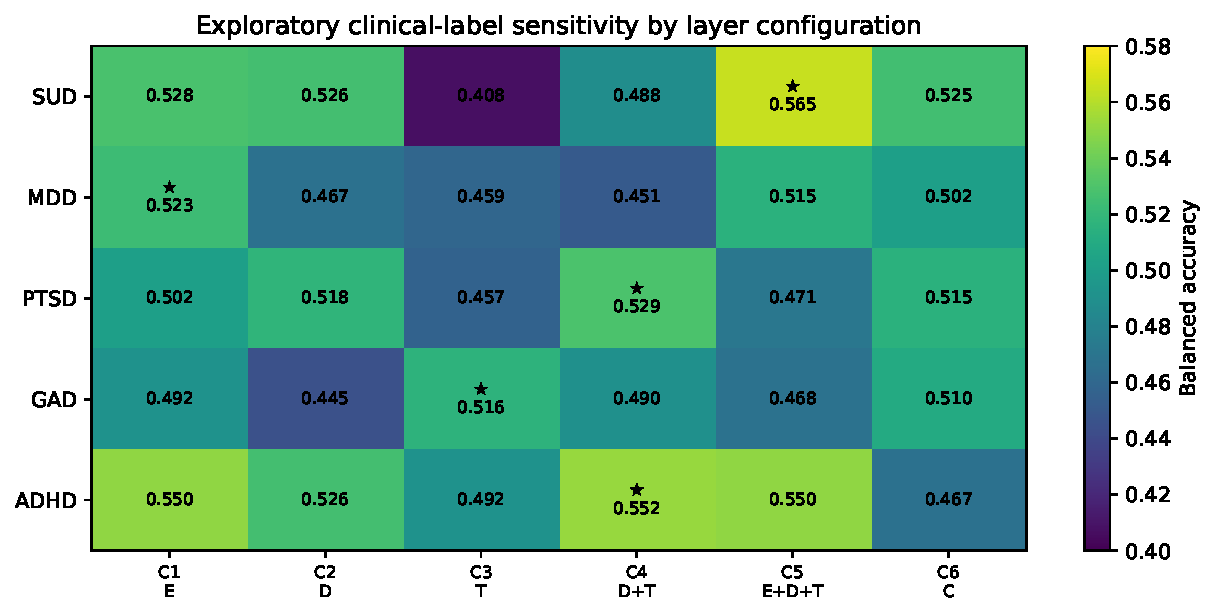
\includegraphics[width=0.90\textwidth]{fig06_clinical_sensitivity_heatmap.pdf}
\caption{Exploratory clinical-label sensitivity heatmap. Stars identify the best balanced-accuracy configuration for each diagnosis. These results do not establish diagnostic biomarkers.}
\label{fig:clinical_heatmap}
\end{figure*}

\begin{figure}[!t]
\centering
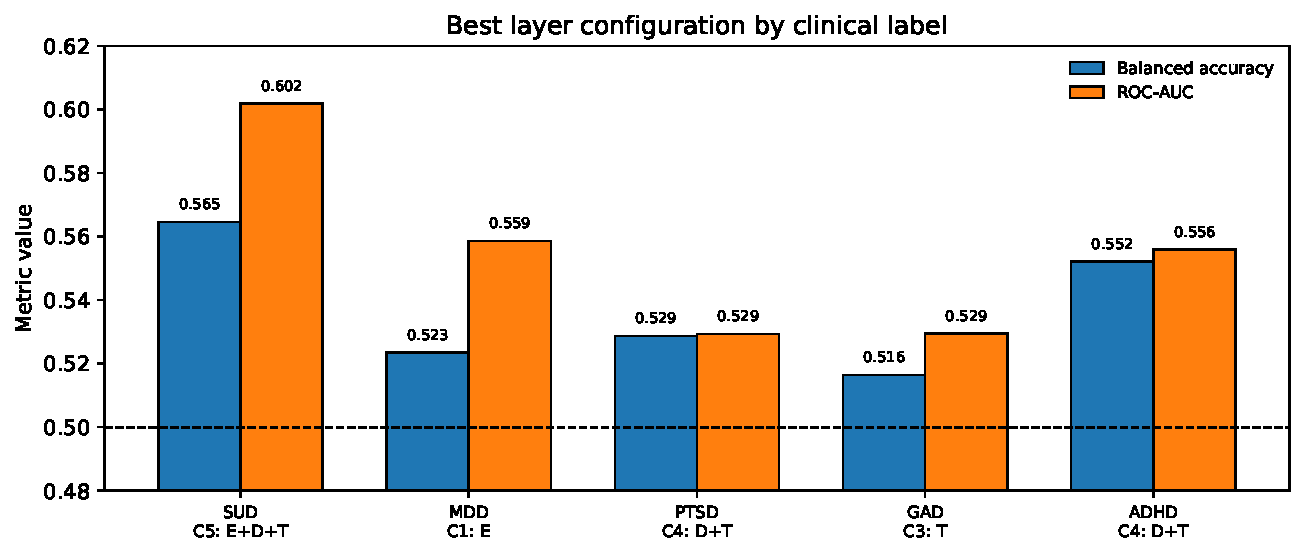
\includegraphics[width=\columnwidth]{fig07_clinical_best_layer_dual_metric.pdf}
\caption{Best clinical-label configuration for each diagnosis. The best layer combination varies across labels, supporting target-dependent layer utility.}
\label{fig:clinical_best_fig}
\end{figure}

The absolute clinical values are modest. The highest balanced accuracy is 56.46\% for SUD using $E+D+T$. Therefore, the correct interpretation is weak clinical-label sensitivity, not detection.

\subsection{Comorbidity-Adjusted Exploratory Models}
Exploratory comorbidity-adjusted logistic models included layer score, other diagnoses, comorbidity count, age, sex, and assigned sex where available. Selected rows are shown in Table~\ref{tab:adjusted}. ADHD showed the clearest adjusted pattern: $E$ had an uncorrected layer-score $p=0.0432$ and $E+D+T$ had $p=0.0094$. SUD had an uncorrected topological association, but the coefficient was negative. Because FDR correction and permutation inference were not completed, these associations are used only to guide interpretation.

\begin{table}[!t]
\caption{Selected Comorbidity-Adjusted Layer-Score Models}
\label{tab:adjusted}
\centering
\footnotesize
\begin{tabular}{llccc}
\hline
Target & Layer score & Coef. & $p$ & Model AUC \\
\hline
SUD & C3: $T$ & -1.7417 & 0.0201 & 0.6699 \\
ADHD & C1: $E$ & 2.1289 & 0.0432 & 0.7215 \\
ADHD & C5: $E+D+T$ & 2.6385 & 0.0094 & 0.7301 \\
\hline
\end{tabular}
\end{table}


\subsection{Layer Redundancy}
Pairwise CKA values were low to moderate. The largest value was $\mathrm{CKA}(E,D)=0.3058$. All other reported CKA values were lower: $E$--$T=0.0299$, $E$--$C=0.0738$, $D$--$T=0.0174$, $D$--$C=0.1858$, and $T$--$C=0.0314$. This supports non-equivalence of the layer spaces. CCA saturated for several pairs, which is expected in high-dimensional low-sample regimes; CKA and ridge cross-predictability are therefore treated as the more conservative indicators.

\begin{table}[!t]
\caption{Selected Pairwise Layer Redundancy Values}
\label{tab:redundancy}
\centering
\footnotesize
\begin{tabular}{lcc}
\hline
Layer pair & Linear CKA & Ridge $R^2$ \\
\hline
$E \rightarrow D$ & 0.3058 & 0.1005 \\
$E \rightarrow T$ & 0.0299 & -0.1434 \\
$E \rightarrow C$ & 0.0738 & 0.0362 \\
$D \rightarrow T$ & 0.0174 & -3.8916 \\
$D \rightarrow C$ & 0.1858 & -1.5910 \\
$T \rightarrow C$ & 0.0314 & -0.1659 \\
\hline
\end{tabular}
\end{table}


\begin{figure}[!t]
\centering
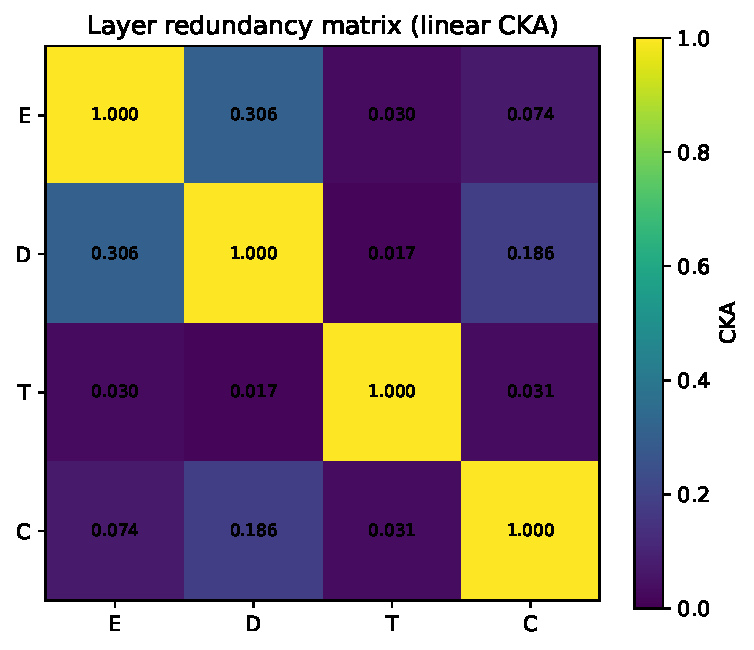
\includegraphics[width=\columnwidth]{fig08_layer_redundancy_cka.pdf}
\caption{CKA redundancy matrix. Low-to-moderate CKA values indicate that feature families are not trivial linear duplicates.}
\label{fig:cka}
\end{figure}

\subsection{Claim Strength}
Fig.~\ref{fig:claim_ladder} summarizes the evidence boundary. Completed analyses support operational layer utility, feature-block validity, and exploratory covariate-adjusted clinical sensitivity. They do not support diagnostic biomarkers because permutation-FDR inference was not completed.

\begin{figure*}[!t]
\centering
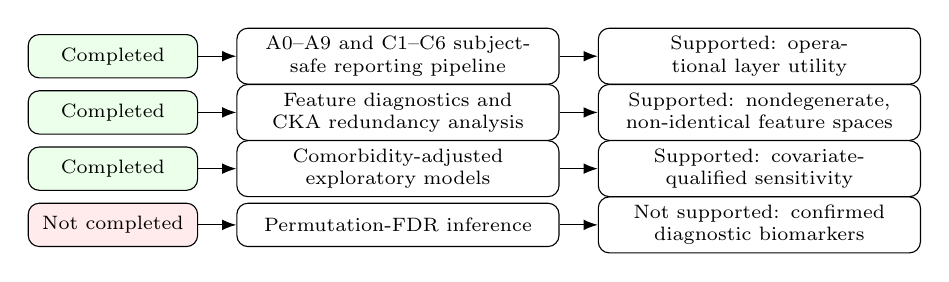
\begin{tikzpicture}[font=\scriptsize, node distance=0.18cm]
\tikzstyle{box}=[draw, rounded corners, align=center, inner sep=3pt, minimum height=0.55cm]
\node[box, fill=green!8, text width=0.16\textwidth] (a1) {Completed};
\node[box, text width=0.32\textwidth, right=0.04\textwidth of a1] (a2) {A0--A9 and C1--C6 subject-safe reporting pipeline};
\node[box, text width=0.32\textwidth, right=0.04\textwidth of a2] (a3) {Supported: operational layer utility};
\node[box, fill=green!8, text width=0.16\textwidth, below=0.15cm of a1] (b1) {Completed};
\node[box, text width=0.32\textwidth, right=0.04\textwidth of b1] (b2) {Feature diagnostics and CKA redundancy analysis};
\node[box, text width=0.32\textwidth, right=0.04\textwidth of b2] (b3) {Supported: nondegenerate, non-identical feature spaces};
\node[box, fill=green!8, text width=0.16\textwidth, below=0.15cm of b1] (c1) {Completed};
\node[box, text width=0.32\textwidth, right=0.04\textwidth of c1] (c2) {Comorbidity-adjusted exploratory models};
\node[box, text width=0.32\textwidth, right=0.04\textwidth of c2] (c3) {Supported: covariate-qualified sensitivity};
\node[box, fill=red!8, text width=0.16\textwidth, below=0.15cm of c1] (d1) {Not completed};
\node[box, text width=0.32\textwidth, right=0.04\textwidth of d1] (d2) {Permutation-FDR inference};
\node[box, text width=0.32\textwidth, right=0.04\textwidth of d2] (d3) {Not supported: confirmed diagnostic biomarkers};
\foreach \x/\y in {a1/a2,a2/a3,b1/b2,b2/b3,c1/c2,c2/c3,d1/d2,d2/d3}{\draw[-{Latex[length=1.8mm]}] (\x) -- (\y);}
\end{tikzpicture}
\caption{Evidence ladder used to constrain the manuscript claims. This paper supports operational distinctness and exploratory clinical-label sensitivity, not clinical deployment or biomarker validation.}
\label{fig:claim_ladder}
\end{figure*}

\section{Discussion}
\subsection{Main Finding}
The main finding is that ARSPI-Net layers are target-dependent. Affective classification is strongest for embedding-containing configurations and remains comparable to a conventional band-power baseline. Clinical-label sensitivity peaks in different layer combinations. Redundancy analysis shows that the layers are not identical feature spaces. Together, these observations support operational distinctness.

\subsection{Why This Is Not Merely an Ablation Table}
In many architecture papers, ablation is used only to prove that every module improves the final result. That is not the finding here. Adding $C$ to $E+D+T$ does not improve affective balanced accuracy. $T$ and $C$ alone are weak affective classifiers. Yet the clinical-label matrix shows that $T$ and $D+T$ can be the highest-sensitivity configurations for GAD, PTSD, and ADHD. This demonstrates why endpoint accuracy alone is an insufficient audit of a staged biomedical architecture.

\subsection{Clinical Interpretation}
The clinical findings are deliberately bounded. Values between approximately 51\% and 56\% balanced accuracy are not diagnostic performance. They are weak-signal indicators that clinical labels perturb representations differently. This is compatible with transdiagnostic heterogeneity: psychiatric labels may be expressed through distributed temporal, dynamical, and spatial organizations rather than one universal EEG feature space.

\subsection{Comparison to IEEE-Style EEG Papers}
The manuscript follows the rigor expected in recent IEEE EEG papers by separating architecture, feature definitions, ablation, subject-safe evaluation, clinical caution, and limitations. The contribution differs from performance-first SNN/GNN classifiers~\cite{gong2023sglnet,klepl2023ad} and multimodal biomedical models~\cite{guo2025mma}: the objective is not to claim state-of-the-art accuracy, but to determine whether a staged neuromorphic architecture has empirically distinct measurement layers.

\section{Limitations}
Permutation-FDR inference was not completed in the current run; therefore, clinical-label findings remain exploratory. The clinical labels are comorbid and cannot be interpreted as disorder-specific mechanisms from these analyses alone. The reservoir embedding in this corrected run achieved 46.96\% balanced accuracy, not higher values reported in earlier dissertation-stage summaries; this manuscript uses the corrected reporting pipeline as source of truth. Finally, the results are based on one clinical affective EEG dataset and require external validation.

\section{Conclusion}
This paper evaluated whether ARSPI-Net layers are redundant feature transformations or operationally distinct measurement layers. The corrected ablation shows target-dependent utility: embedding-containing configurations are strongest for affective classification, whereas exploratory clinical-label sensitivity peaks in different layer combinations. Low-to-moderate CKA values support non-equivalence of the layer spaces. The methodological contribution is the operational-distinctness analysis itself: staged biomedical signal architectures should be evaluated by what each layer measures, not only by whether each layer increases a single endpoint accuracy.

\section*{Acknowledgment}
The authors acknowledge that the reporting outputs used in this draft are privacy-preserving. Prediction-level artifacts use hashed subject identifiers only.

\balance
\bibliographystyle{IEEEtran}
\bibliography{references}

\end{document}
